%
% Use the standard article template.
%
\documentclass{article}

% The geometry package allows for easy page formatting.
\usepackage{geometry}
\geometry{letterpaper}

% Load up special logo commands.
\usepackage{doc}

% Package for formatting URLs.
\usepackage{url}

% Packages and definitions for graphics files.
\usepackage{graphicx}
\usepackage{float}
\usepackage{epstopdf}
\DeclareGraphicsRule{.tif}{png}{.png}{`convert #1 `dirname #1`/`basename #1 .tif`.png}

%
% Set the title, author, and date.
%
\title{Nashville Instagram Filter}
\author{Anders Dahl}
\date{}

%
% The document proper.
%
\begin{document}

% Add the title section.
\maketitle

% Add an abstract.
\abstract{

    The purpose of this research is to identify and replicate the effects used by Instagram's Nashville filter. The Nashville filter utilizes level \cite{website:levels}, brightness \cite{website:brightness}, and color \cite{website:colors} adjustments to give it a low contrast, high exposure, and warm temperature. It adds a pastel, slightly pink and pleasant palette to your photo. \cite{website:photodoto} I attempted to recreate these adjustments in my own custom filter, but at the end, there were still some slight differences.
}

% Add various lists on new pages.
\pagebreak
\tableofcontents

% Start the paper on a new page.
\pagebreak

%
% Body text.
%
\section{Introduction}
\label{introduction}

The purpose of this research is to identify and replicate the effects used by Instagram's Nashville filter. The Nashville filter utilizes level \cite{website:levels}, brightness \cite{website:brightness}, and color \cite{website:colors} adjustments to give it a low contrast, high exposure, and warm temperature. It adds a pastel, slightly pink and pleasant palette to your photo. \cite{website:photodoto} The result can be seen below:

\begin{figure}[H]
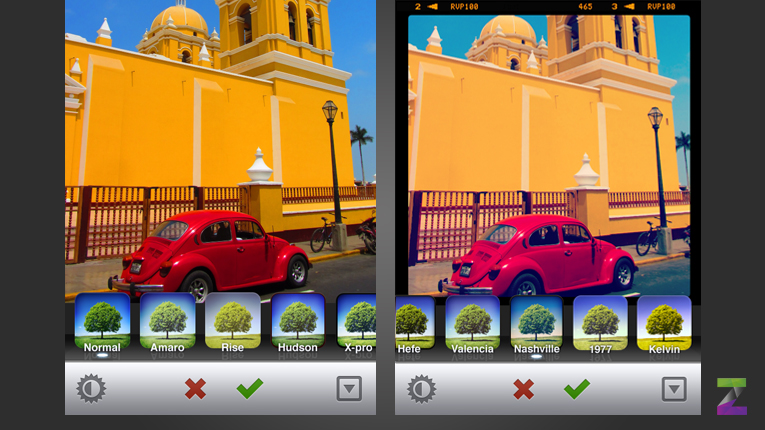
\includegraphics[width=\linewidth]{Nashville.jpg}
\caption{Instagram's Nashville Filter.}
\end{figure}

I was able to roughly map out what the Instagram filter was doing by
looking at the histogram of the RGB channels of the before and after photos. The article  'How to make Instagram Filters in Photoshop: Nashville and 1997' was also an invaluable source that gave me a general direction of what to look for. In the end, I concluded that some level, brightness, and color adjustments were present. The color adjustments caused a tint resembling a maize-like-color.

I attempted to recreate the Nashville filter by altering the contrast, gamma, tint (color ratios), and input color to try to get a similar effect. I compared the original, instagram, and custom image side-by-side with their respective color channels on display in a histogram. Using this technique, I was able to figure out what I needed to adjust in order to get a closer fit. My custom filter was able to get close to the Instagram filter, but there were still some slight differences.

\pagebreak

\section{Methods}

\subsection{Level Adjustment}

\begin{figure}[H]
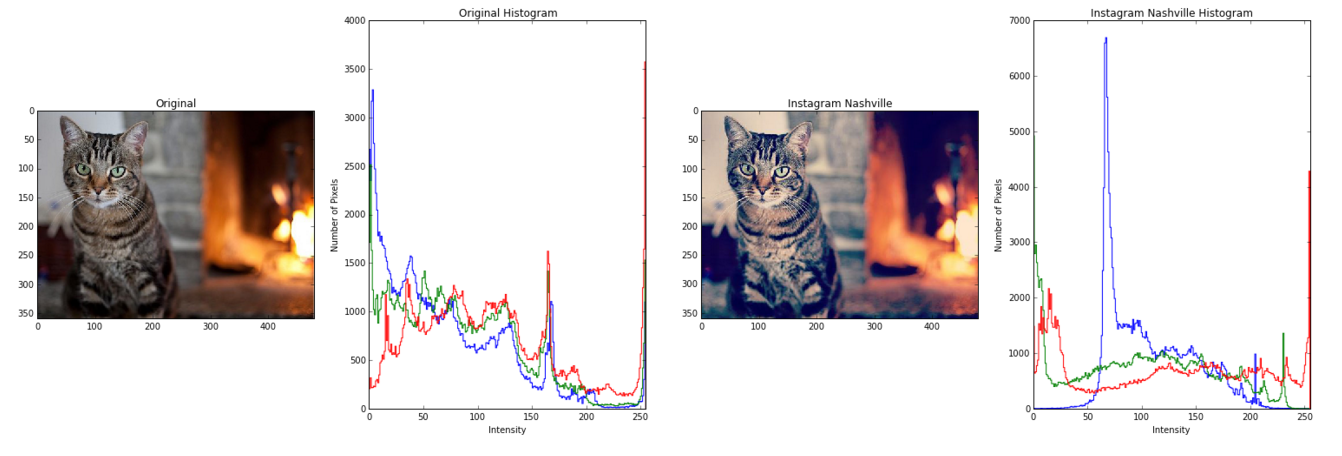
\includegraphics[width=\linewidth]{color_input_adjustment.png}
\caption{Color Input Adjustments.}
\label{fig:colorInputAdjustment}
\end{figure}

You can adjust the level to correct the tonal range and color balance of an image by adjusting the intensity. \cite{website:levels} The input intensity of the Instagram Nashville filter is different; hence, a level adjustment seems to be occurring. This is illustrated in figure \ref{fig:colorInputAdjustment}. For example, the blue channel spikes upwards at an intensity of about 65 compared to the spike at 0 in the original photo. The green channel has a similar adjustment, but it is not as substantial. After testing on multiple images, it seemed like the input color adjustments were close to the following: \cite{website:photodoto}
\begin{description}
\item[Red Channel] 0
\item[Green Channel] 18
\item[Blue Channel] 88
\end{description}

\subsection{Brightness Adjustments}
Instagram's Nashville filter adjusts the brightness across the board. The intensity of each channel has increased.  In figure \ref{fig:colorInputAdjustment} we see that many more pixels are in a higher intensity region.

\pagebreak
\subsection{Color Ratio Adjustments}

\begin{figure}[H]
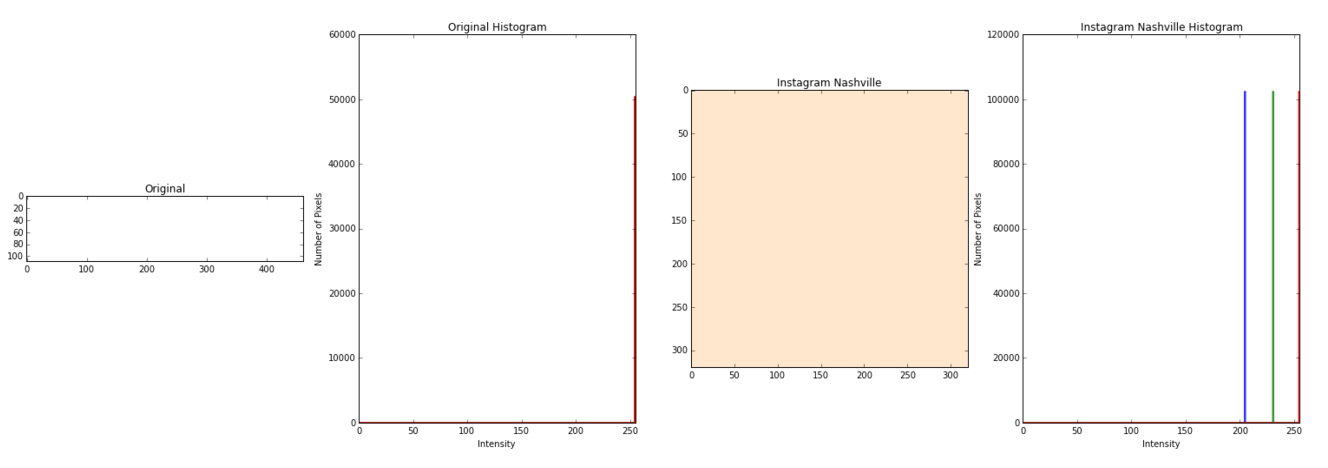
\includegraphics[width=\linewidth]{color_ratio_adjustment.png}
\caption{Color Ratio Adjustment}
\label{fig:colorRatioAdjustment}
\end{figure}
If we run Instagram's Nashville filter on a white image, we notice that a maize-colored tint has been applied. The above figure \ref{fig:colorRatioAdjustment} shows this. The Instagram histogram clearly show the shift in the red, green, and blue channels. The maize color is close to \#F6D8AC or RGB(246, 216, 172). We can approximate the ratio change for each channel by diving those values by the white, RGB(255, 255, 255).
\begin{description}
\item[Red Channel Ratio Change] .965
\item[Green Channel Ratio Change] .847
\item[Blue Channel Ratio Change] .6745
\end{description}

\pagebreak

\section{Code}

After analyzing the photos, I started coding. After some manual testing I found three functions that were essential in creating a similar custom filter. I used the Skimage Exposure library with Python to achieve this, and all my code can be found in the iPython Notebook provided.

\begin{enumerate}
\item Contrast
\item Gamma
\item Tint and Input Color
\end{enumerate}

\subsection{Contrast}

\begin{figure}[H]
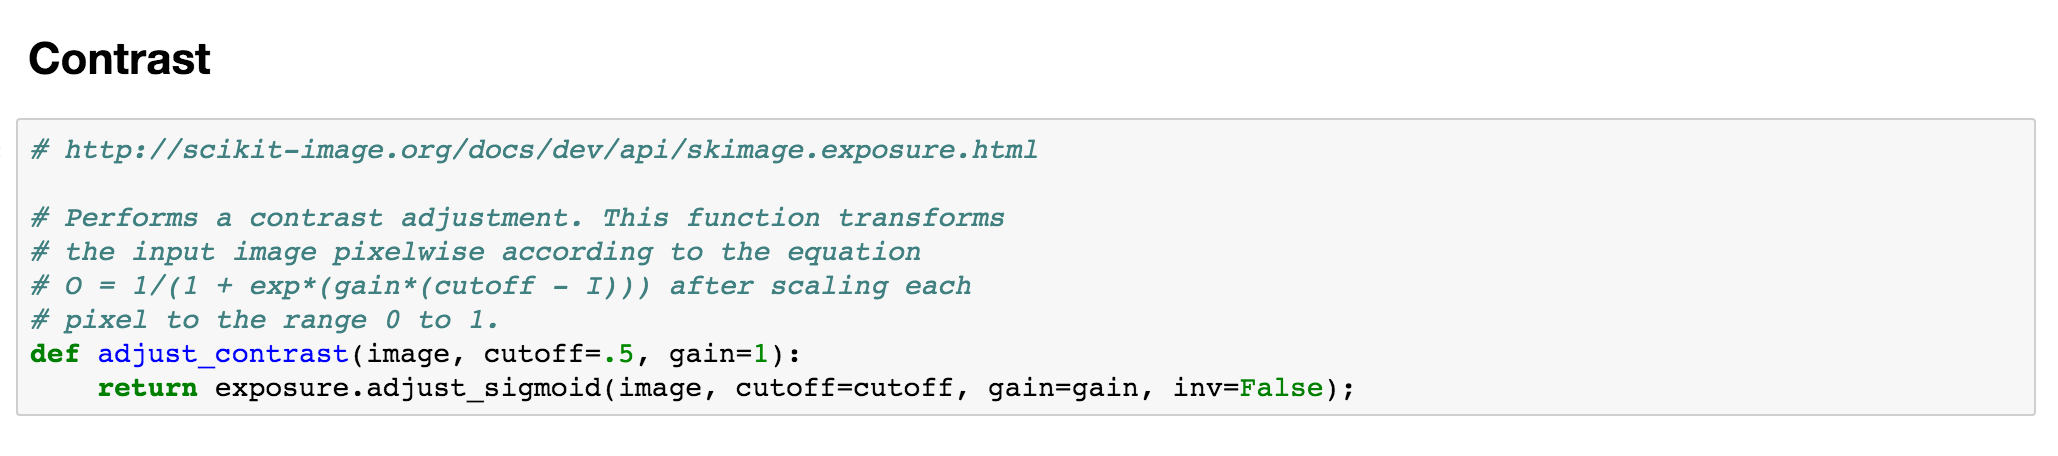
\includegraphics[width=\linewidth]{contrast.png} \caption{Contrast Adjustment}
\label{fig:contrastAdjustment}
\end{figure}

Run a contrast adjustment. This function transforms the input image pixelwise according to the equation O = 1/(1 + exp*(gain*(cutoff - I))) after scaling each pixel to the range 0 to 1. \cite{website:exposure} It can can be used to adjust the brightness and sharpness of the image. After some experimenting, I found that a gain of 8 worked well. This brightens the image.

\subsection{Gamma}

\begin{figure}[H]
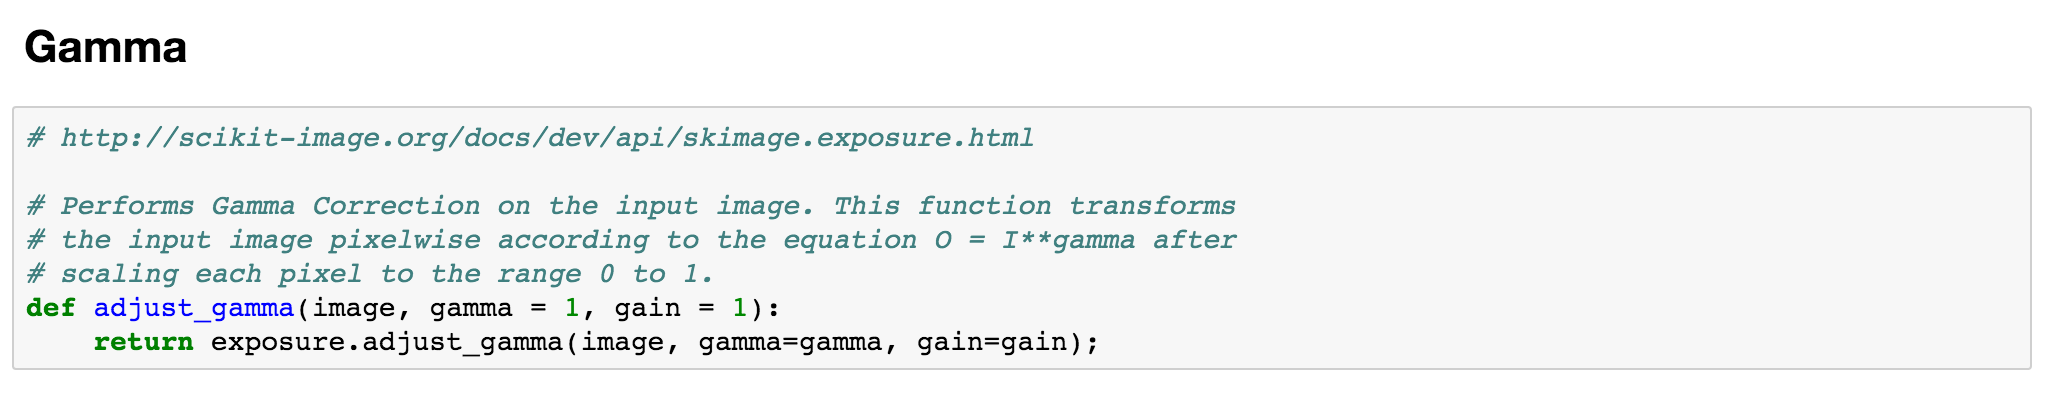
\includegraphics[width=\linewidth]{gamma.png} \caption{Gamma Adjustment}
\label{fig:gammaAdjustment}
\end{figure}

Performs Gamma Correction on the input image. Also known as Power Law Transform. This function transforms the input image pixelwise according to the equation O = I**gamma after scaling each pixel to the range 0 to 1. \cite{website:exposure} It can can be used to adjust the brightness and sharpness of the image. After some experimenting, I found that a gamma of .68 worked well. This brightens the image.

\subsection{Tint and Input Color}

\begin{figure}[H]
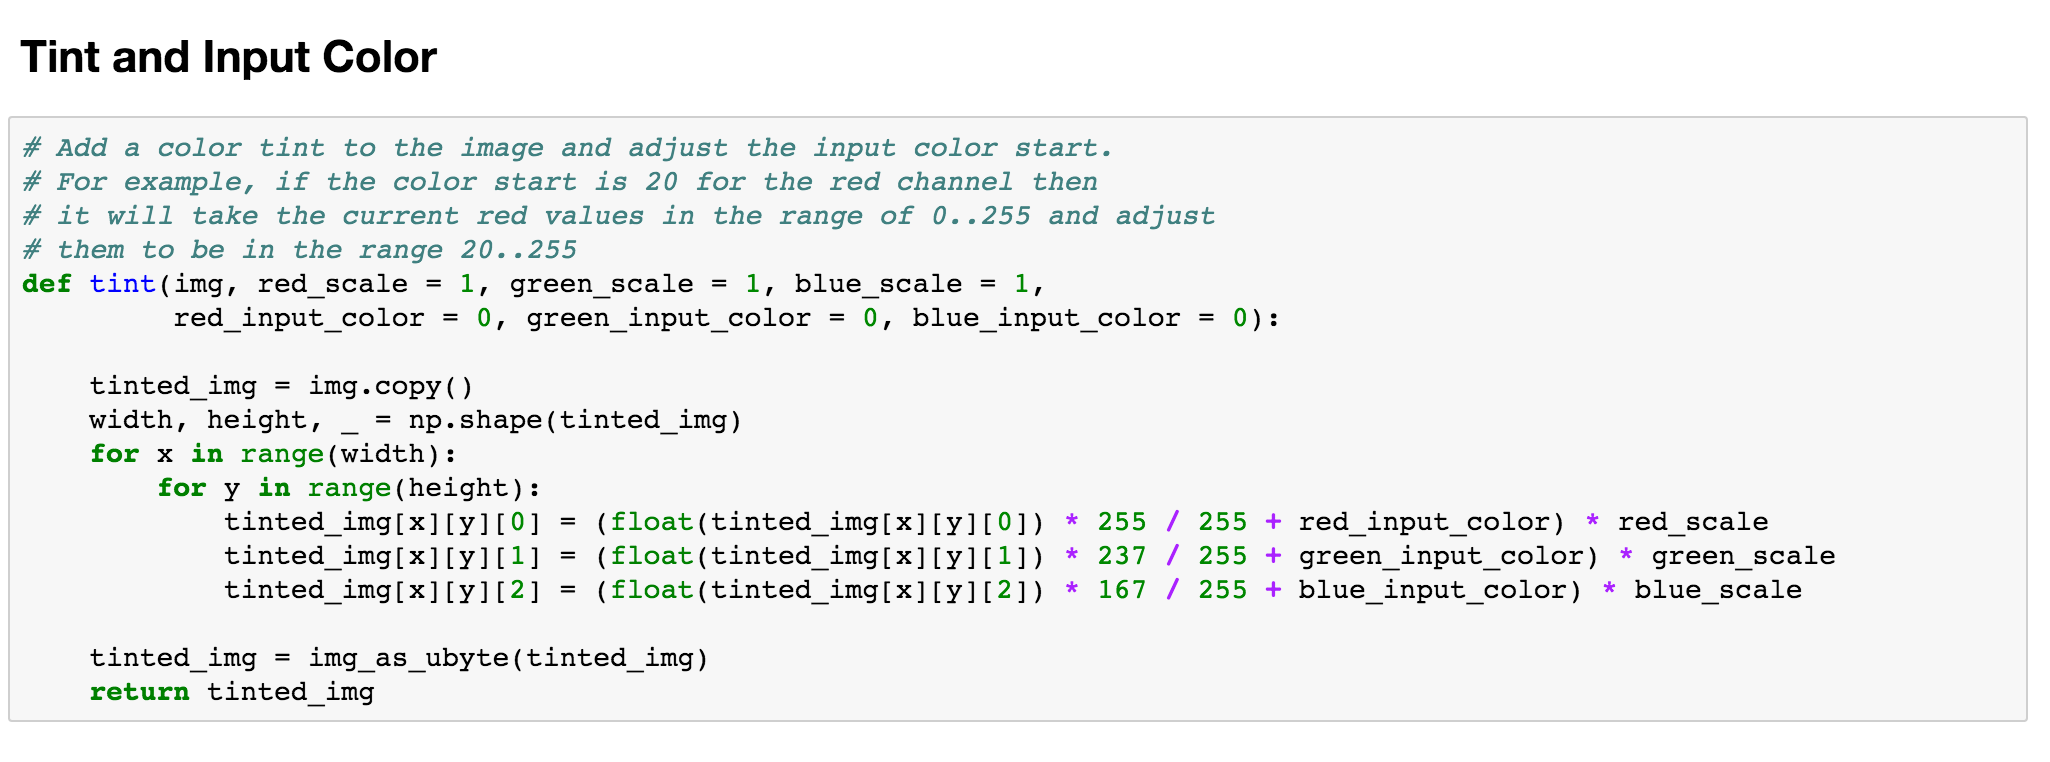
\includegraphics[width=\linewidth]{tint_and_input_color.png} \caption{Tint and Input Color Adjustment}
\label{fig:gammaAdjustment}
\end{figure}

This function adds a color tint to the image and adjusts the input color. For example, if the color input is 20 for the red channel then it will take the current red values in the range of 0..255 and adjust them to be in the range 20..255. In our case, we want to run the function with the tint ratio and color input values calculated previously in the methods section. This will give us something close to a maize-colored \#F6D8AC with the appropriate input color values.

\section{Results}

The results are formatted as original, Instagram, and custom. Here are the results:

\begin{figure}[H]
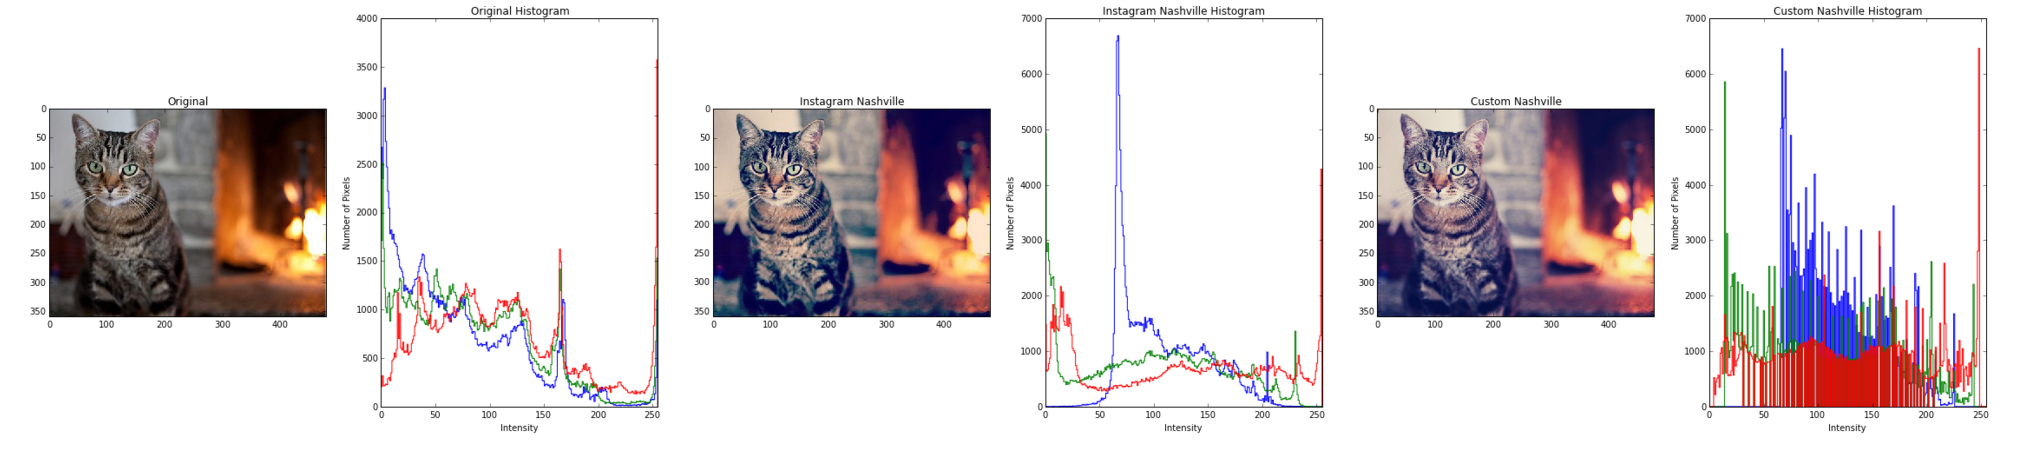
\includegraphics[width=\linewidth]{result1.png} \caption{Result 1}
\label{fig:result1}
\end{figure}

\begin{figure}[H]
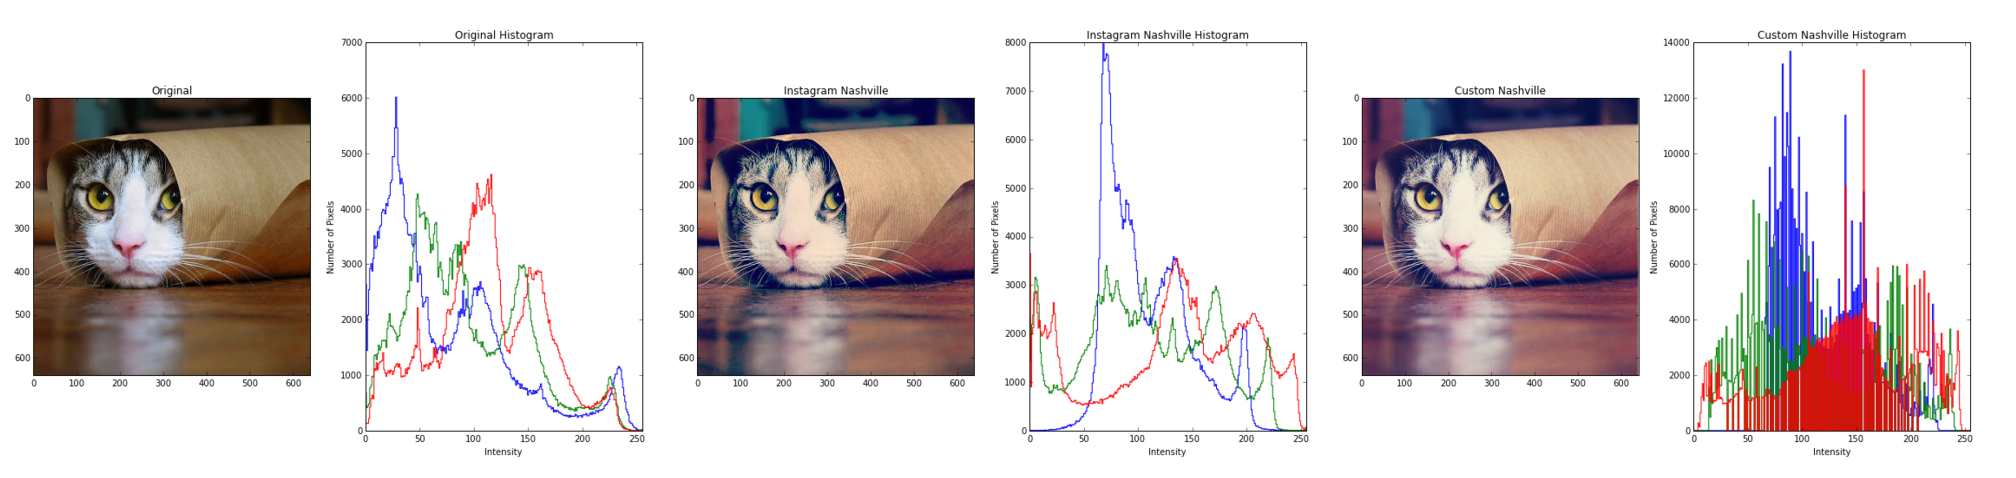
\includegraphics[width=\linewidth]{result2.png} \caption{Result 2}
\label{fig:result2}
\end{figure}

\begin{figure}[H]
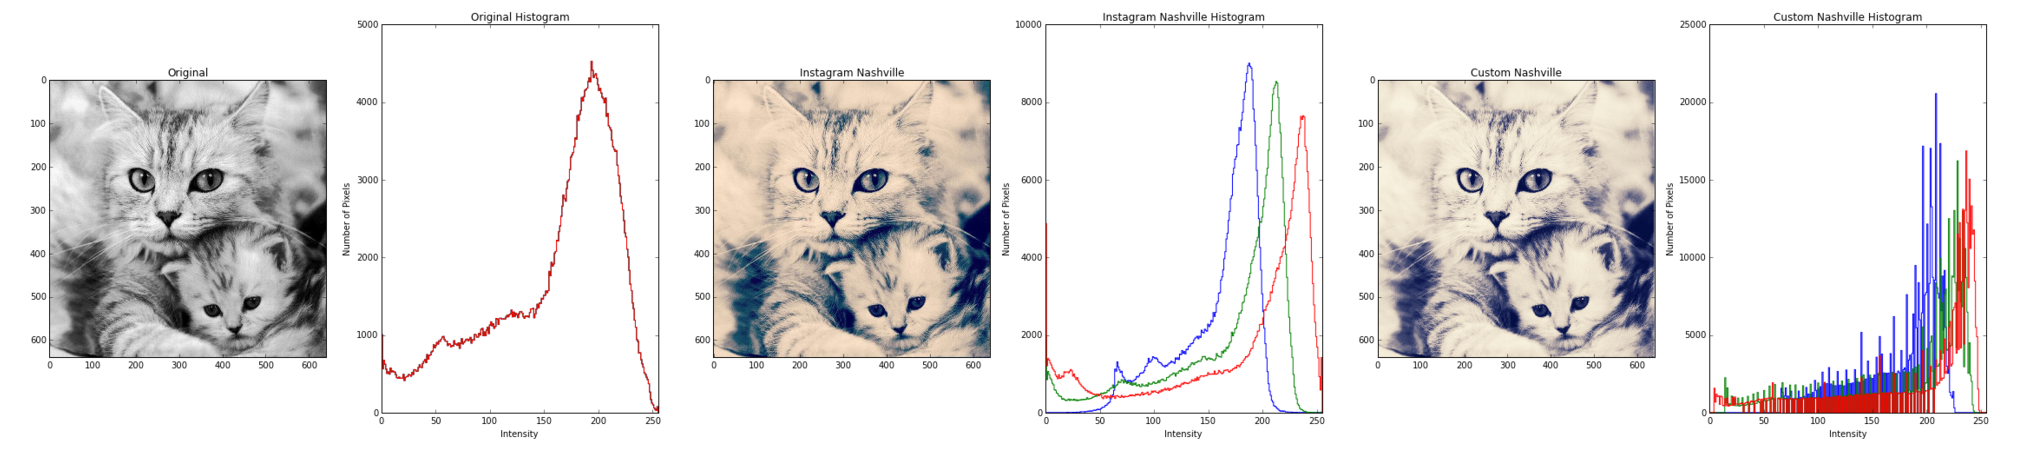
\includegraphics[width=\linewidth]{result3.png} \caption{Result 3}
\label{fig:result3}
\end{figure}

\begin{figure}[H]
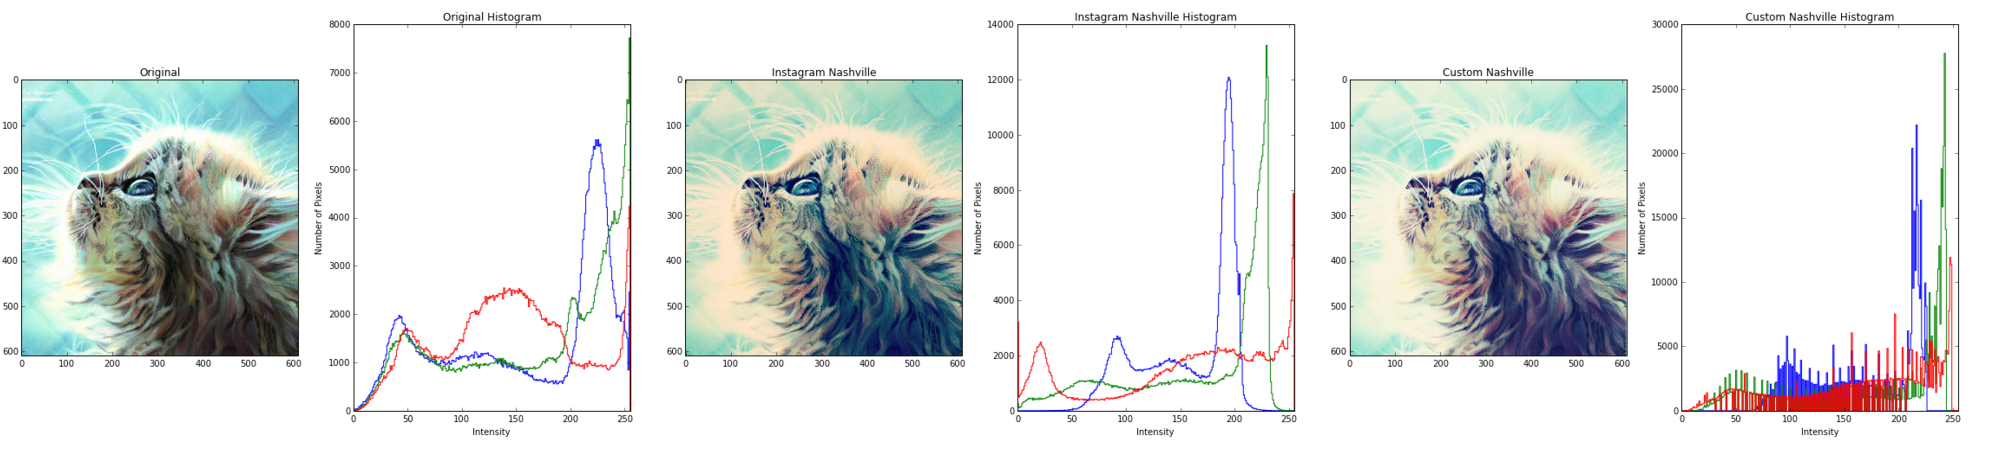
\includegraphics[width=\linewidth]{result4.png} \caption{Result 4}
\label{fig:result4}
\end{figure}

\section{Discussion}
In conclusion, it was hard to get a perfect match with Instagram's Nashville filter. There's a lot more going on under the hood than what I have implemented. Even though my custom filter gets close, it is by no means an exact match. I hypothesize that Instagram does some color adjustments based on the intensity level. My tint and input level function is the same across the intensity range, and that makes for a much less complicated function.

\pagebreak
\bibliography{InstagramFilter}
\bibliographystyle{acm}

\end{document}
